% omci.tex:

\chapter{OPTICAL MAMMOGRAPHY CO-IMAGER (OMCI)} % all caps please
\label{chap:omci}
% should I include the abstract as the first paragraph of the chapter? That way it feels like a stand-alone piece?  

% challenge and application
%innovation and significance

\section{Introduction} %significan
\label{chap:omci:introduction}
Breast cancer is the most commonly diagnosed cancer in women worldwide with an estimated 1,918,030 new cases in 2022 in the United States alone~\cite{Siegel2022}. X-ray mammography is the primary breast cancer screening technique~\cite{Secretan2015} used for early detection to reduce mortality rates~\cite{Tabar2003}. Despite its recommendation for screening, x-ray mammography suffers from a high false-positive diagnostic rate~\cite{Tabar2003, Elmore1998}. The technique lacks both strong structural contrast between healthy and tumor tissue and the ability to quantify tissue functions to assess benign versus malignancy~\cite{Leff2008}. These limitations have led researchers to investigate using diffuse optical tomography (DOT) techniques to characterize the breast tumor's physiology to lower false-positive diagnoses. 

Unlike x-ray mammography, DOT is an imaging modality that uses non-ionizing near-infrared (NIR) radiation to yield three-dimensional (3-D) maps of the optical properties of illuminated tissue~\cite{Boas2001, Dehghani2009, Yamada2014, Hoshi2016}. Biological tissues' primary absorbers in the spectral window from around 600 to 1000~nm have relatively low absorption, allowing NIR light to penetrate through centimeters of tissues~\cite{Gibson2005}. This allows the quantification of physiological properties such as hemoglobin concentration, blood volume, and blood oxygen saturation~\cite{Leff2008, Boas2001}. Malignant tumors generally demand a greater blood supply than their surrounding tissues, leading to increased light absorption that can be delineated using spectroscopy and imaging methods, making DOT particularly useful for breast cancer imaging diagnosis~\cite{Wang2022, Vavadi2014, Flexman2013, Choe2009, Taroni2005}. Additionally, the low spatial resolution of DOT~\cite{Li2010} can be improved by a multi-modal approach with x-ray mammography~\cite{Zimmermann2017, Deng2015, Deng2015a, Fang2009a}. DOT images are known for low spatial resolution largely caused by the high scattering properties of biological tissues~\cite{Boas2001}. The high scattering present in the breast tissue redirects photons to traverse large overlapping probing volumes before their detection, greatly reducing the locality of the measurements and resulting in blurry images. Mathematically, this is reflected as the severe ill-posedness of the inverse problem. Parallel-plate compression of breast tissues has been used in an x-ray mammography scan to minimize overlapping tissues and has also been explored for a number of standalone~\cite{Choe2009, Culver2003} and multi-modal DOT breast imaging systems~\cite{ZhuReview2020, Fang2009a, Krishnaswamy2012}. Obtaining breast surface information to aid quantitative analysis of imaging data has garnered interest from a number of applications, including digital breast tomosynthesis (DBT)~\cite{Rodriguez2017} and magnetic resonance imaging (MRI) scans~\cite{Pallone2014, Ortiz2012}.

For multi-modal DOT systems, the 3-D shape of the breast can be estimated using the structural imaging modality such as DBT~\cite{Fang2011} or MRI~\cite{Brooksby2006}. When a 3-D imaging modality is not available, two-dimensional (2-D) mammography~\cite{Deng2015a} has also been used to provide the shape information. In such case, a simple way to recover a 3-D breast surface is to extrude the 2-D breast contour along the compression axis~\cite{Kruger2013, Kalbhen1999}, or sweep the 2-D breast contour along the contour line extracted from an orthogonal view~\cite{Kita1998}. These methods either rely on assumptions about the 3-D location of certain features (e.g. mamilla position) or assume a constant curvature of the breast along the sweeping direction. For more accurate reconstructions of tissue optical properties, especially near the surface, measuring 3-D breast surface accurately can be greatly beneficial.

Accurately acquiring breast 3-D surface shapes has gained clinical acceptance due in large part to the plastic and reconstructive surgery communities~\cite{Chang2015, Losken2005}. The two prominent techniques for 3-D breast surface imaging are stereophotogrammetry and laser scanning~\cite{Yang2015}. Stereophotogrammetry works by overlaying multiple images of an object taken from different view angles and triangulating the location of the object based on matching features in the multiple images~\cite{Ju2016, Galdino2002, FangOSA2012}. In addition to requiring multiple cameras to increase accuracy~\cite{Henseler2012}, this technique is also heavily influenced by lighting conditions since features need to be extracted from multiple viewpoints~\cite{Henseler2011}. Another limitation is the ``ptosis error'' seen during scanning of ptotic or larger breasts~\cite{Nahabedian2003}. This arises due to the small field of view of stereophotogrammetry systems, leading to inaccuracies in breast surface and volume estimations due to the portions of the breast that are not illuminated. Laser scanning is a surface imaging technique in which rays from a laser beam are reflected off an object and detected by a detector~\cite{Kovacs2006}. Although laser-based acquisition systems can produce more accurate surfaces~\cite{Kovacs2006b}, these systems tend to be expensive~\cite{Kovacs2007, Koch2011} and require the need for very precise setups~\cite{Thomson2009}. Recently, the use of patterned-lasers and orientation-sensitive detectors has led to an increase in portable 3-D laser scanning devices~\cite{Kuzminsky2012}. While low-cost laser-based depth sensors have been widely deployed in game consoles such as Xbox or PlayStation, they are only designed to achieve relatively low spatial accuracy compared to dedicated 3-D scanners. Still, patterned-laser-based surface acquisition systems generally require a minimum scanner-to-target distance of 35~cm~\cite{Ametek2002, Artec3D2022}. Additionally, their typical housing is too large to fit between mammography compression plates~\cite{Artec3D2022, Pallone2014}. Bulky instrumentation and long minimum working distance requirements make stereophotogrammetry and laser scanning techniques infeasible in the confined, low-light mammography setting. 

Another widely used 3-D surface acquisition technique is structured light imaging (SLI)~\cite{Yang2020, Zhang2018}. SLI works by illuminating an object with two-dimensional spatially varying patterns with a projector and capturing images from the illuminated object using cameras~\cite{Geng2011}. The distortion of the specially designed patterns provides information regarding the shape of the object. Calibration of the camera-projector system is easily done by capturing images of a known planar pattern (e.g. a checkerboard). With the ability to use off-the-shelf components, a simple setup with a single projector and camera, and a robust and simple calibration method, SLI is positioned to provide accurate, fast, and cost-effective breast surface scanning~\cite{Yang2020}. However, similar to most patterned-laser surface scanners, commercially available SLI systems have long minimal working distance requirements and large assemblies that cannot readily fit within the confined mammography compression plates~\cite{Zhang2018, Rodriguez2017}.

In this work, we have developed a low-profile dual-camera SLI breast shape acquisition system specifically tailed for use in the confined space between parallel breast compression plates. This system can be incorporated with standalone DOT breast scanners or multi-modal DOT systems combined with mammography or DBT, with a minimal scanner-to-target distance between 10 and 15~cm. In the following sections, we first describe the design of the SLI breast scanner and detail the methods for adaptive illumination for subject-specific skin tones as well as approaches to reduce specular reflection from the compression plates. We then compare several traditional surface acquisition methods that leverage mammography images against our SLI-based breast surface acquisition system and quantify the impact of improved breast surface acquisition on the recovery of breast lesions using a series of simulations.



\section{Methods}
\label{chap:omci:methods}
Here, we first briefly describe a mammography-mimicking parallel-plate transmission breast DOT system, designed to be used as either a standalone DOT scan of a compressed breast or combined with separately acquired mammography or DBT images in a multi-modality data analysis~\cite{Fang2009, Deng2015}. Then we elaborate on the SLI breast surface acquisition sub-system and surface data processing pipeline. This custom SLI system is designed to be compact, low-cost, and specifically tailored towards the low-light and space-confined mammography compression settings. Next, we compare this approach with a number of alternative breast shape acquisition methods, including single-axis and dual-axis contour-line extrusion methods, and create benchmarks to quantify the surface accuracy improvement of the proposed method. Finally, we compare results from a series of DOT image reconstructions based on simulated data with various surface acquisition methods to further quantify the impact of breast surface accuracy, especially for the accurate recovery of tumors embedded at various depths.

%%% Subsection %%%
\subsection{Wide-field parallel-plate transmission breast DOT system}

\begin{figure}
	\begin{center}
	\subfigure[]{\label{fig:mammography_top}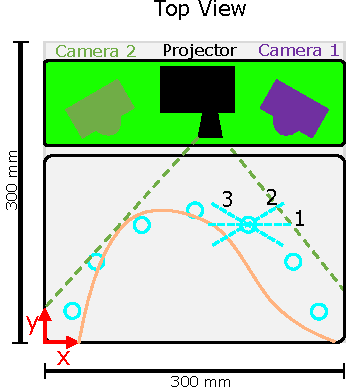
\includegraphics[height=5cm]{mammography_top.pdf}}
	\subfigure[]{\label{fig:mammography_side}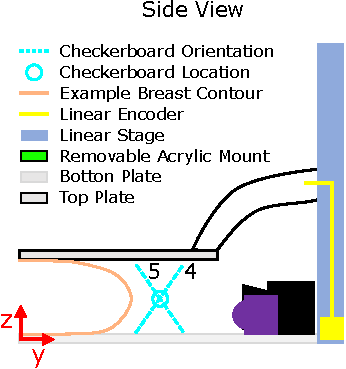
\includegraphics[height=5cm]{mammography_side.pdf}}
	\subfigure[]{\label{fig:mammography_setup}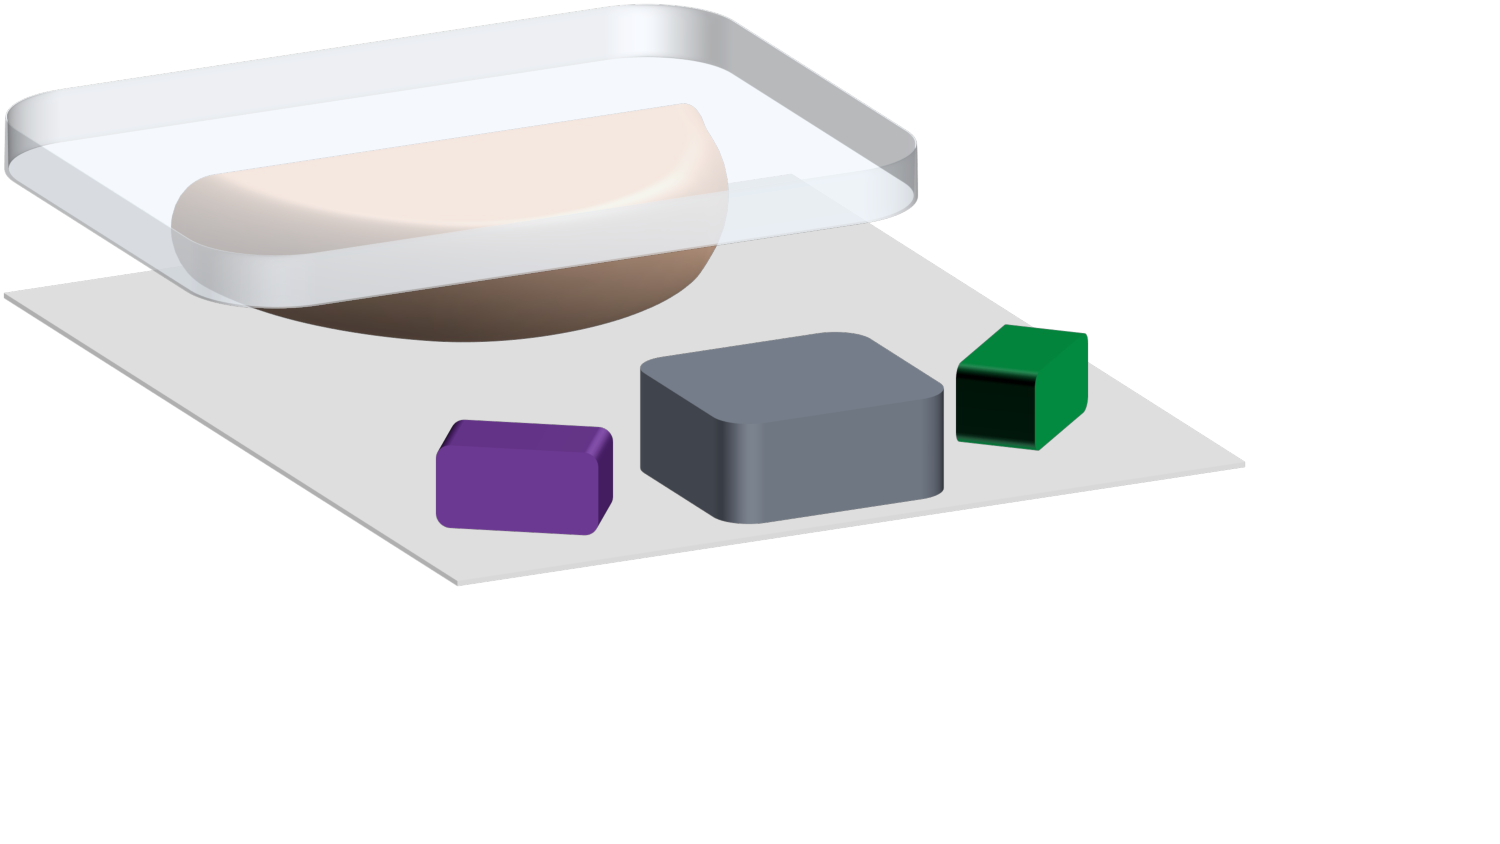
\includegraphics[width=5cm]{sli_model.pdf}}
	\end{center}
	\caption{ (a) Top-view of the breast compression compartment -- upper: SLI system; bottom: horizontal cross-section (orange line) of the compressed breast with blue circles indicating the placement of the checkerboard used for system calibration. Numbers 1-5 indicate the 5 board orientations repeated at each location for calibration. (b) Side-view of the breast compression plates, showing the linear translation stage (blue bar on the right) and a linear encoder (in yellow), and  (c) 3-D rendering of the SLI system, an acrylic bottom plate and an acrylic compression paddle (top). } 
	\label{fig:mammographysetup}
\end{figure} 

A parallel-plate transmission optical tomography system with the capability of imaging a breast with mammography-mimicking compression was built where the proposed SLI system is embedded between the compression plate to provide accurate measurement of the breast surface [Fig.~\ref{fig:mammography_setup}]. The breast is compressed by a pair of acrylic plates, with one plate mounted at the stationary end of a linear stage (BiSlide, Velmex, Bloomfield, NY, USA). An acrylic mammography compression paddle is mounted on the moving stage of the linear stage, allowing for a plate separation ranging from 300~mm (fully released) to 0~mm (fully closed) using a 2-phase stepper motor (Oriental Motors, Braintree, MA, USA). A linear encoder (ETI Systems, Carlsbad, CA, USA) is connected between the pair of compression plates to measure their separation. The entire breast compression assembly is mounted on a rotatory table (Lintech, Monrovia, CA, USA), controlled by a foot paddle to permit mammography-like lateral-oblique compression. This breast DOT design specifically enables registration of structural information from separately acquired mammography scans with the DOT images using the methods detailed in our previous studies~\cite{Deng2015}. The details of this breast DOT system will be described in a separate publication.%CITE Omci paper here when it is available

%%% Subsection %%%
\subsection{Dual-camera SLI breast surface scanning system}\label{sec:sli}
The main focus of this report is to characterize and evaluate the SLI-based breast surface acquisition sub-system. This low-profile SLI scanner has a dimension of 30$\times$10$\times$4.8~cm$^3$, and is fixated on a stationary compression plate, on the side facing the patient's breast [Fig.~\ref{fig:sli_setup}]. It consists of a central projector (P2-B DLP Pico Projector, AAXA Technologies, Irvine, CA, USA) and two USB cameras (C525, Logitech, Lausanne, Switzerland) to reconstruct a 3-D surface of the compressed breast. The SLI scanner is designed to have a relatively short scanner-to-target distance, typically less than 15~cm, and a vertical profile of less than 3~cm to permit scanning breasts with a wide range of sizes. A laptop is used to control the data acquisition, including illumination pattern generation, projection, camera image acquisition, and translation stage control via an interface written in MATLAB (R2017b, Mathworks, Natick, MA, USA).

Gray-code based binary patterns~\cite{Inokuchi1984} are sequentially illuminated onto the breast surface and captured using both USB cameras. These patterns are characterized by their pattern order, $P$. A pattern set of $P=3$ results in 3 sequences which are a reflected binary of the previous (``01'', ``0110'', and ``01100110''). Four bar patterns are created for each sequence (a horizontal black and white bar pattern, a vertical black and white bar pattern, and the complimentary pattern of each)~\cite{Sels2019}. The digits correspond to the white (``1'') and black (``0'') bars. In addition, a full-bright (white) and full-dark (black) pattern are added to each pattern set. Thus, a pattern set of $P=3$ results in $4\times P+2$ illumination bar patterns. Complimentary Gray-code based illumination pattern sets are used due to their robustness to decoding errors~\cite{Moreno2012}. The two USB cameras have overlapping field-of-views and sequentially capture images of the breast during each illumination pattern at an exposure time of 250~ms. Dual-camera simultaneous acquisition allows the SLI system to capture the curved surface of breasts of varied sizes without moving components. 

\subsubsection{Special data acquisition considerations}\label{sec:special}
% skin tone
Skin tone differences are known to affect light-based surface reconstruction accuracy, especially in low-light settings. To account for skin tone variations, the normalized illumination patterns are multiplied by a scaling factor $\alpha$ ranging from 0 to 1 to prevent camera saturation. The scaling factor for a camera is calculated prior to data acquisition by first illuminating a full-bright pattern with $\alpha=1$ onto the breast and capturing a single image using the camera. If the maximum pixel value of the captured image is above a preset threshold, $\alpha$ is decreased and the breast is re-illuminated with a full-bright pattern multiplied by the new $\alpha$ value. This procedure is repeated until the maximum pixel value of the captured image is less than 95\% of the camera's maximum allowable pixel value. This entire procedure takes an estimated 8 seconds to complete and is repeated for each camera.

\begin{figure}
	\begin{center}
	\subfigure[]{\label{fig:sli_setup}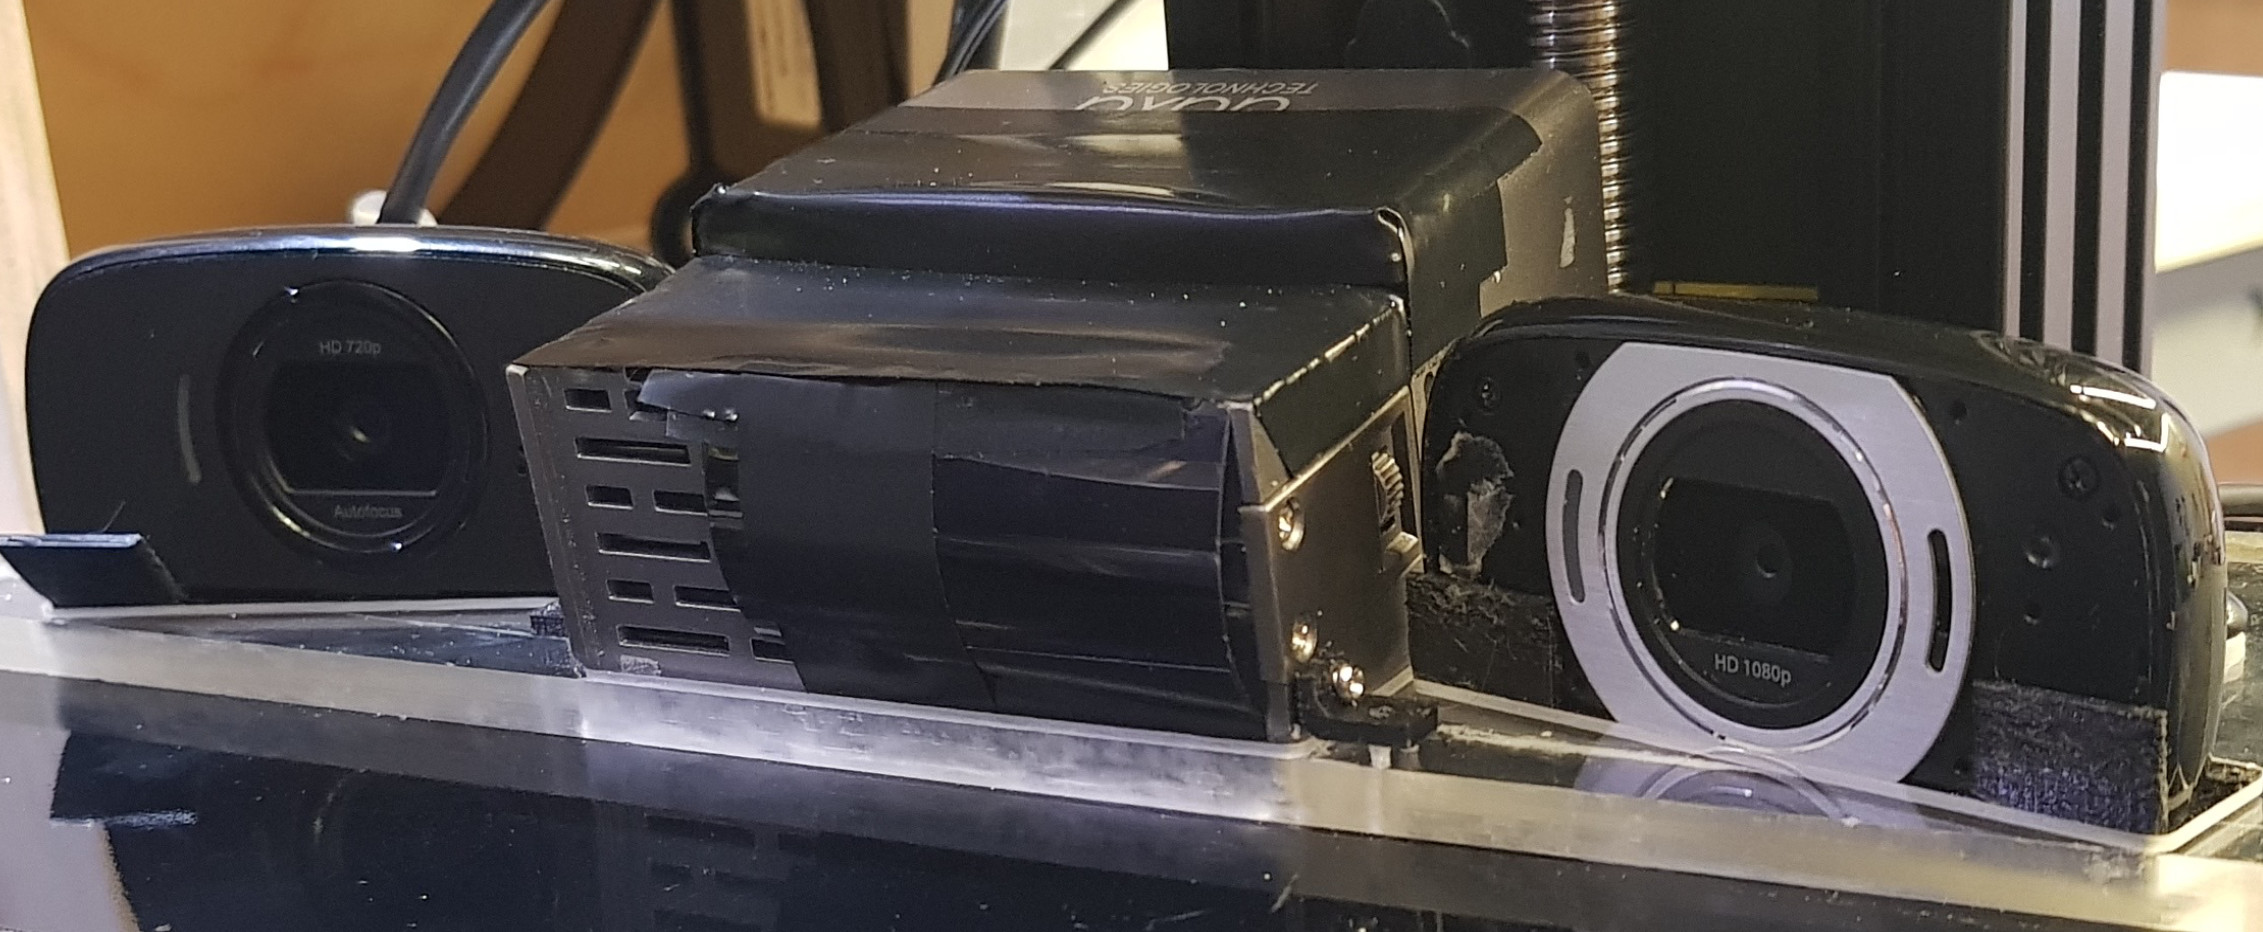
\includegraphics[height=2.4cm]{sli_photo.jpg}}
	\subfigure[]{\label{fig:artifact1}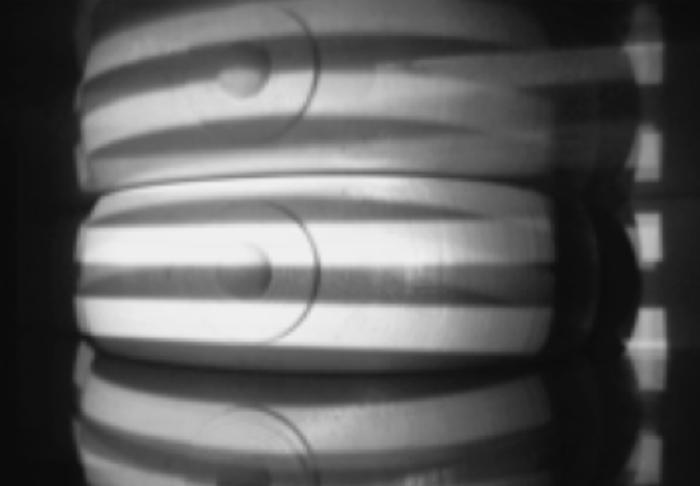
\includegraphics[height=2.4cm]{bars_artifact.png}}
	\subfigure[]{\label{fig:artifact2}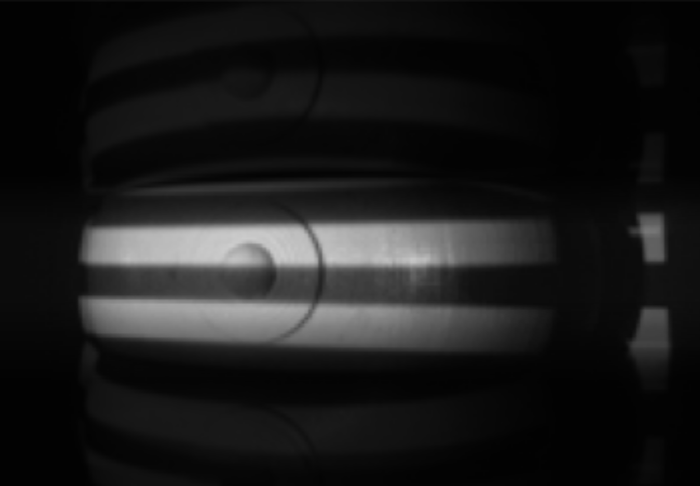
\includegraphics[height=2.4cm]{bars.png}}
	\end{center}
	\caption{(a) Front-view photo of the SLI system. Cameras and projectors are embedded in an acrylic mount to prevent the need for re-calibration. (b) Horizontal bar patterns reflecting off the top compression plate and onto the breast show curved illumination bar artifacts when the scaling factor $\alpha$ is set to 1. In (c), we show the same illumination pattern with thickness-informed masking eliminating the curved bar artifacts by cropping the patterns exceeding the breast surface before projection. Additionally, the scaling factor is automatically calculated to prevent camera saturation.} 
	\label{fig:barartifacts}
\end{figure} 

% encoder-informed masking
Additionally, specular reflections from the acrylic compression plates, shown in Fig.~\ref{fig:artifact1}, can produce vertically mirrored breast surfaces. To minimize such specular reflection, we use dynamic pattern masking based on real-time separation readings provided by a linear encoder. By limiting the vertical span of the illumination patterns, the patterns are projected onto the compressed breast surface without generating strong direct specular reflections from the top and bottom compression plates, as shown in Fig.~\ref{fig:artifact2}.

\subsubsection{SLI system calibration and re-projection errors}
A standard SLI camera-projector calibration is performed prior to image acquisition and is described in detail in~\cite{Moreno2012}. For each camera-projector pair, a checkerboard pattern is fully illuminated in multiple positions and the corner locations are estimated in the projector's default coordinate system using a robust pixel classification algorithm~\cite{Xu2007}. The camera and projector's intrinsic parameters (optical center and focal lengths) are estimated using a calibration method described in~\cite{Zhang2000} by fixing a world coordinate system to the calibration checkerboard plane. 

The projector's extrinsic parameters (rotation and translation from camera to projector) are calculated using a simple stereo camera calibration~\cite{Bouguet2004} that treats the projector as a secondary camera. This results in a rotation matrix and a translation vector relating the camera's coordinates to the projector's coordinates. Once the 3-D coordinates of all the corners of the checkerboard are computed using the camera's (and projector's) intrinsic and extrinsic parameters, the corners are ``reprojected'' onto all the images for which they appear. The re-projection error is defined as the average distance between the re-projected corner locations and the actual corner location. 

\subsubsection{SLI system acquisition}
The same acquisition procedures are used for both calibrating the system and acquiring breast shape measurements (Fig.~\ref{fig:sli_flowchart}). A single acquisition refers to the image capture of all illumination patterns by both cameras. Camera-projector calibration requires an acquisition at each checkerboard position. During breast measurements, the acquisition is preceded by the determination of the saturation scaling factor $\alpha$ and masking of the patterns. Patterns during calibration are not masked since the calibration is done with the system fully uncompressed. 

\begin{figure}
    \begin{center}
    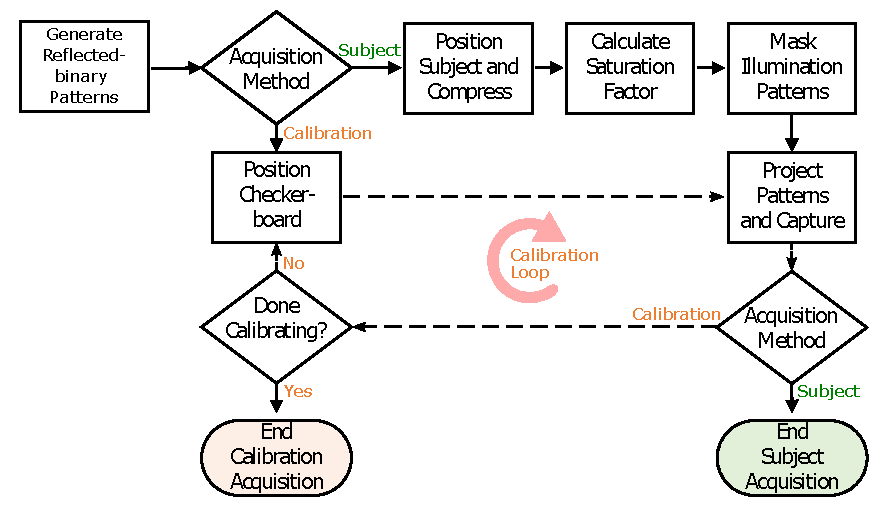
\includegraphics[width=.9\textwidth]{sli_flowchart.pdf}
    \end{center}
    \caption{Flow chart of image acquisition for both subject measurements and system calibration. Subject measurements calculate a saturation scaling factor and mask the illumination patterns prior to projecting patterns. System calibration measurements do not mask the illumination patterns and project at full intensity. The calibration loop (dashed lines) is repeated for each location and orientation of the calibration checkerboard.} 
    \label{fig:sli_flowchart}
\end{figure} 


%%% Subsection %%%
\subsection{Alternative breast surface reconstruction methods for assessing SLI surface accuracy}
To evaluate the accuracy of the SLI system, we compare its output against alternative surface acquisition methods. Each method estimates the surface of a 3-D breast derived from a DBT scan.

\begin{figure}
    \begin{center}
    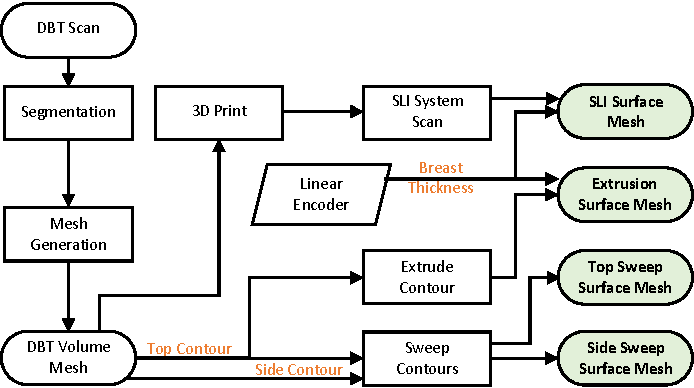
\includegraphics[width=.9\textwidth]{mesh_flowchart2.pdf}
    \end{center}
    \caption{Generation of breast surface meshes using multiple acquisition methods. The DBT volumetric mesh is created from segmented scans. The extrusion surface mesh is created by extruding the top contour to the breast thickness. The top and side contours of the DBT mesh are swept to create top and side surface meshes. The SLI mesh is created by scanning a 3-D printed breast phantom and trimming the resulting point-cloud using the linear encoder measurements. The surface estimation error is calculated for each of the surface meshes by comparing the surface estimations to the DBT mesh. All surface meshes are converted to volumetric meshes for validating the effect of surface estimation methods on inclusion reconstruction.}
    \label{fig:mesh_flowchart}
\end{figure} 

\subsubsection{Reference breast phantom fabrication}
Fig.~\ref{fig:mesh_flowchart} shows the process of creating surface meshes from DBT scans. Scans were obtained from radiology data from The Cancer Genome Atlas (TCGA) breast Invasive Carcinoma collection~\cite{Lingle2016}, available freely through The Cancer Imaging Archive~\cite{Clark2013}. The scan (ID: TCGA-AO-A03M) was chosen due to its large size and complex surface structure, allowing us to highlight the limitations of low field-of-view acquisition methods and as well as traditional shape estimation methods that simply sweep a single breast contour.  Digital Imaging and Communications in Medicine (DICOM) slices were segmented into breast and non-breast regions using ITK-SNAP~\cite{Yushkevich2006}. Segmented slices were converted to a volumetric image and then into a 3-D mesh using a MATLAB toolbox Iso2Mesh~\cite{Fang2009} [Fig.~\ref{fig:mesh_dbt}].

\subsubsection{Single and double contour sweep-based surfaces}
Three alternative surface estimation methods are employed in addition to the SLI surface acquisition method. These three methods use spline models of the DBT breast contours from two different planes (Fig.~\ref{fig:mammographysetup}). The extrusion method creates a surface mesh by extruding the $x/y$ breast contour in the $z$ direction to the thickness of the DBT breast measured by the linear encoder [Fig.~\ref{fig:mesh_extrude}]. The second and third methods utilize a curve-based sweep, in which a profile (shape) follows a path (contour) to create a 3-D model. In the ``top-sweep'' method, the $x/y$ breast contour profile is swept along the $y/z$ breast contour path [Fig.~\ref{fig:mesh_topsweep}]. Similarly, the ``side-sweep'' method uses the $y/z$ breast contour as the profile and the $x/y$ breast contour as the path [Fig.~\ref{fig:mesh_sidesweep}]. In both sweep methods, the profile normal is kept constant.


\begin{figure}
	\begin{center}
	\subfigure[]{\label{fig:mesh_dbt}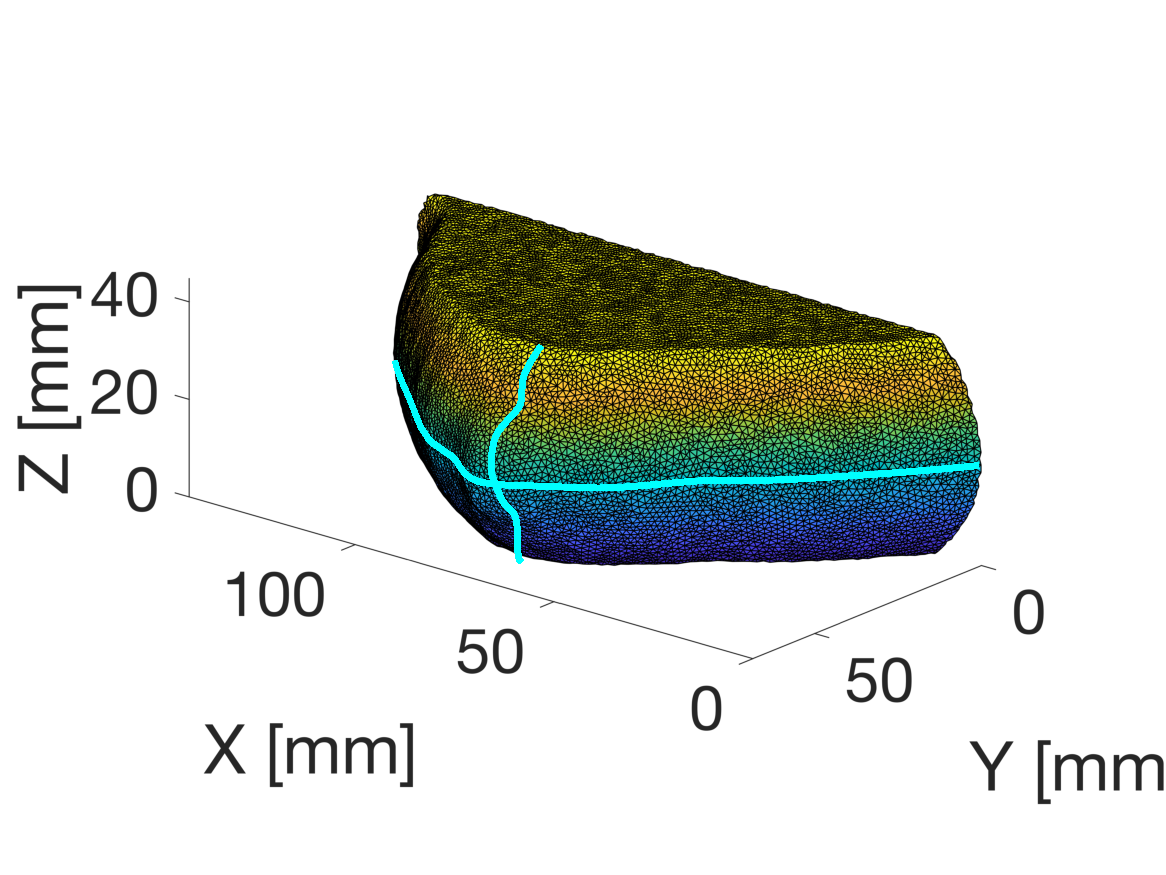
\includegraphics[width=.32\textwidth]{mesh_dbt.pdf}}
	\subfigure[]{\label{fig:mesh_extrude}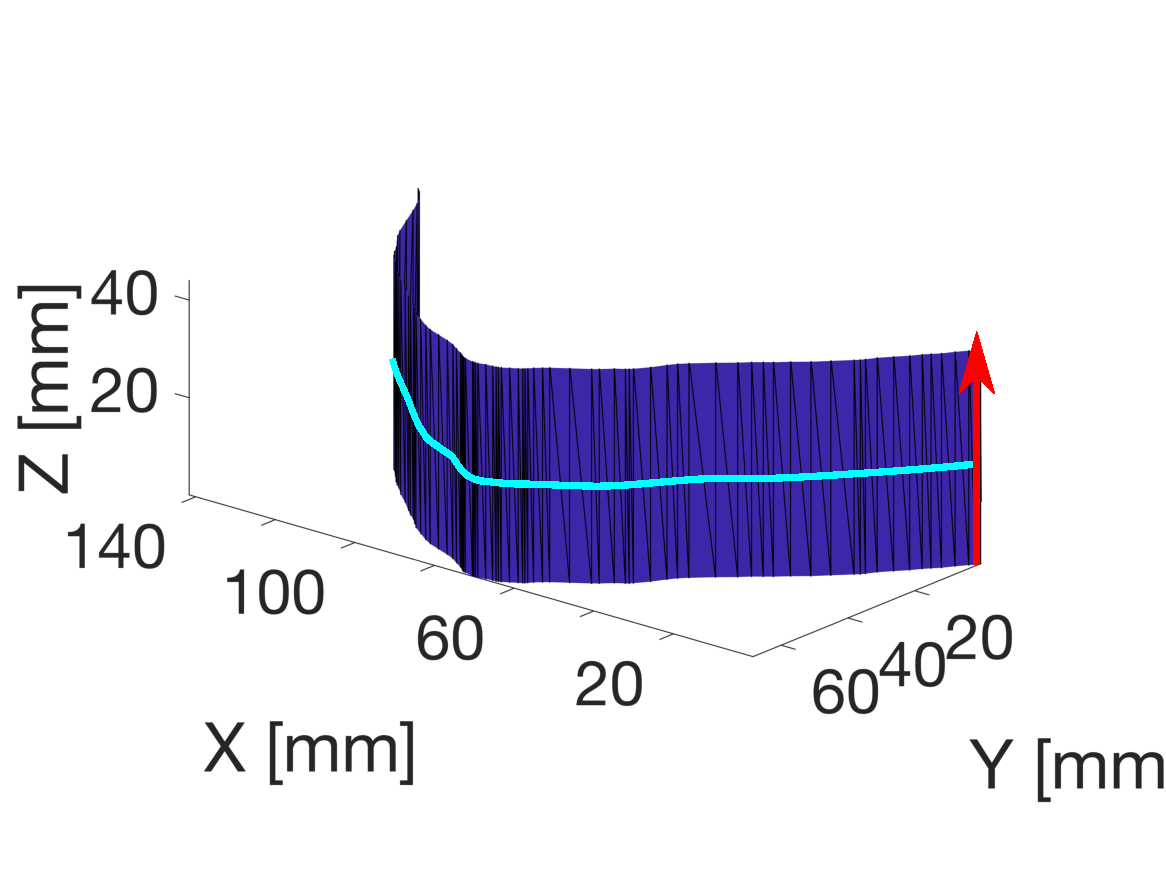
\includegraphics[width=.32\textwidth]{surf_ext.pdf}}
	\subfigure[]{\label{fig:mesh_topsweep}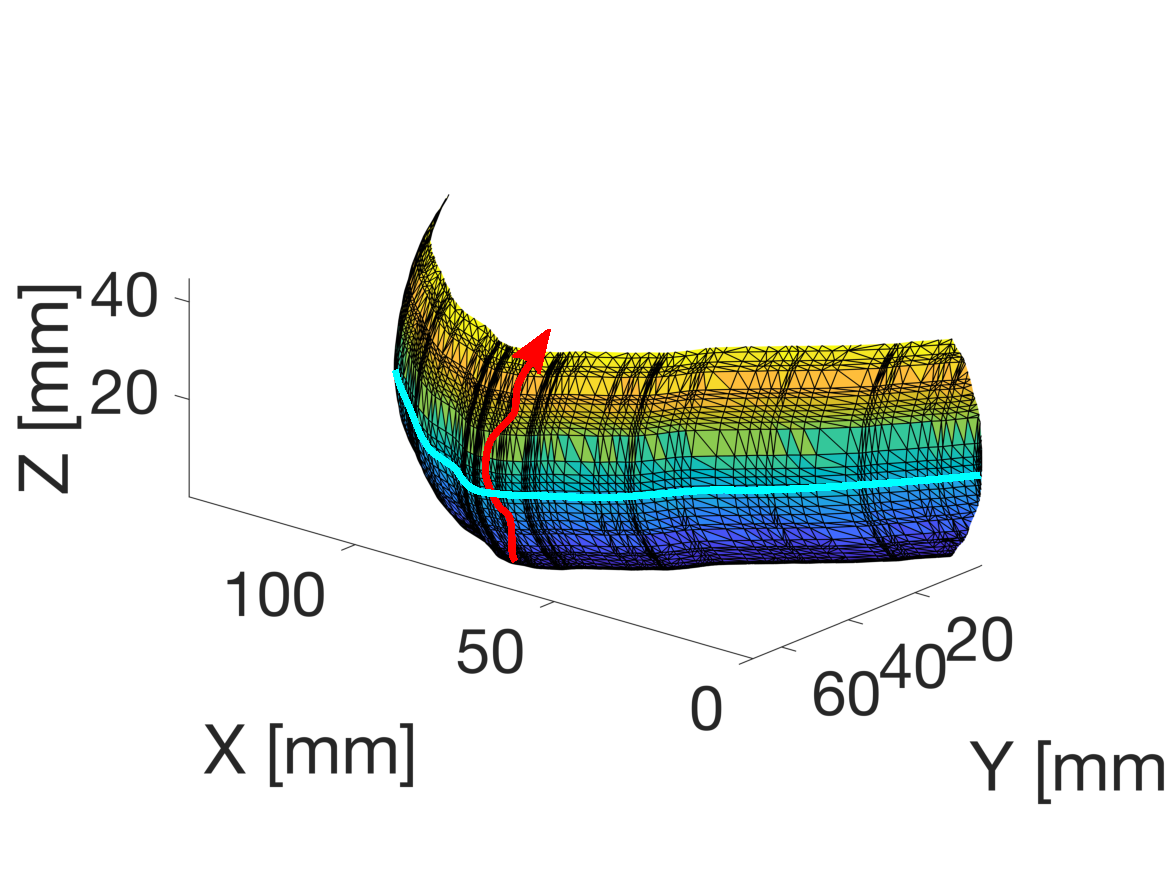
\includegraphics[width=.32\textwidth]{surf_top.pdf}}
	\subfigure[]{\label{fig:mesh_sidesweep}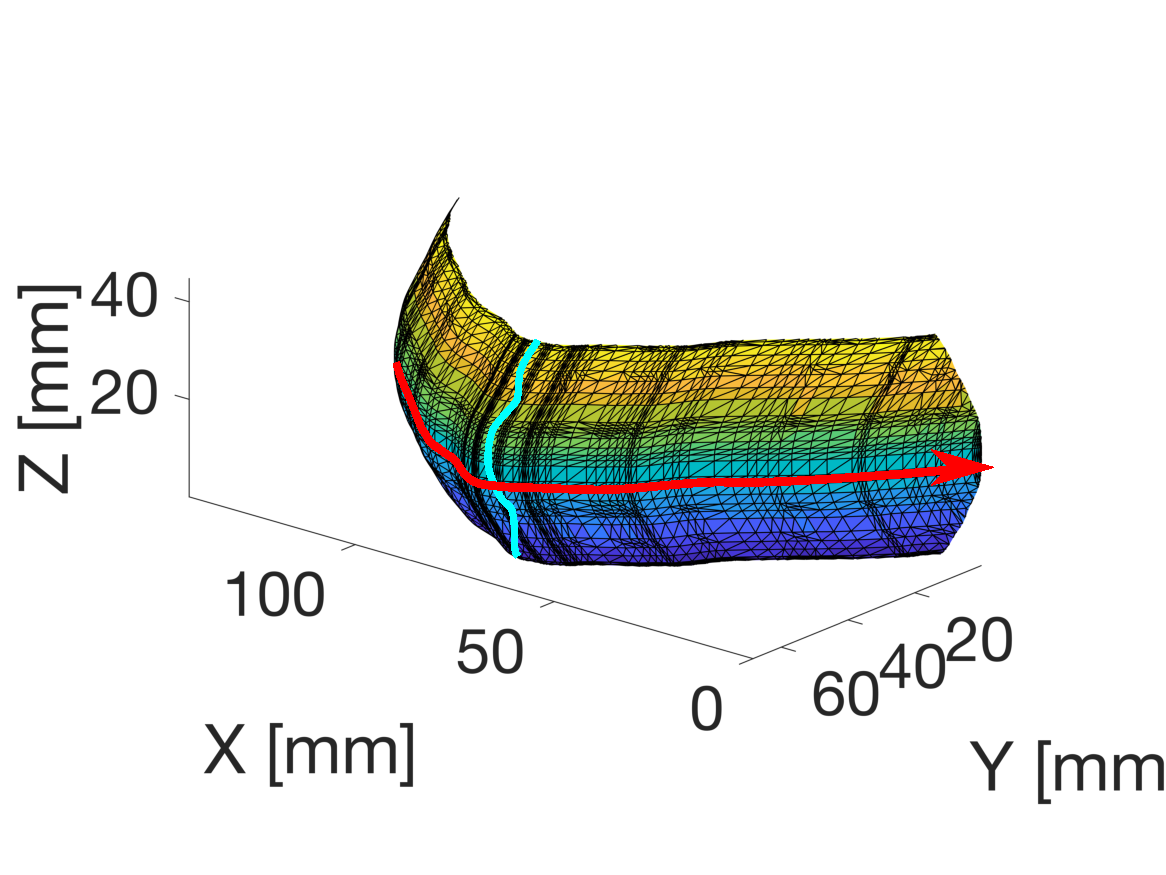
\includegraphics[width=.32\textwidth]{surf_side.pdf}}
	\subfigure[]{\label{fig:pcmergea}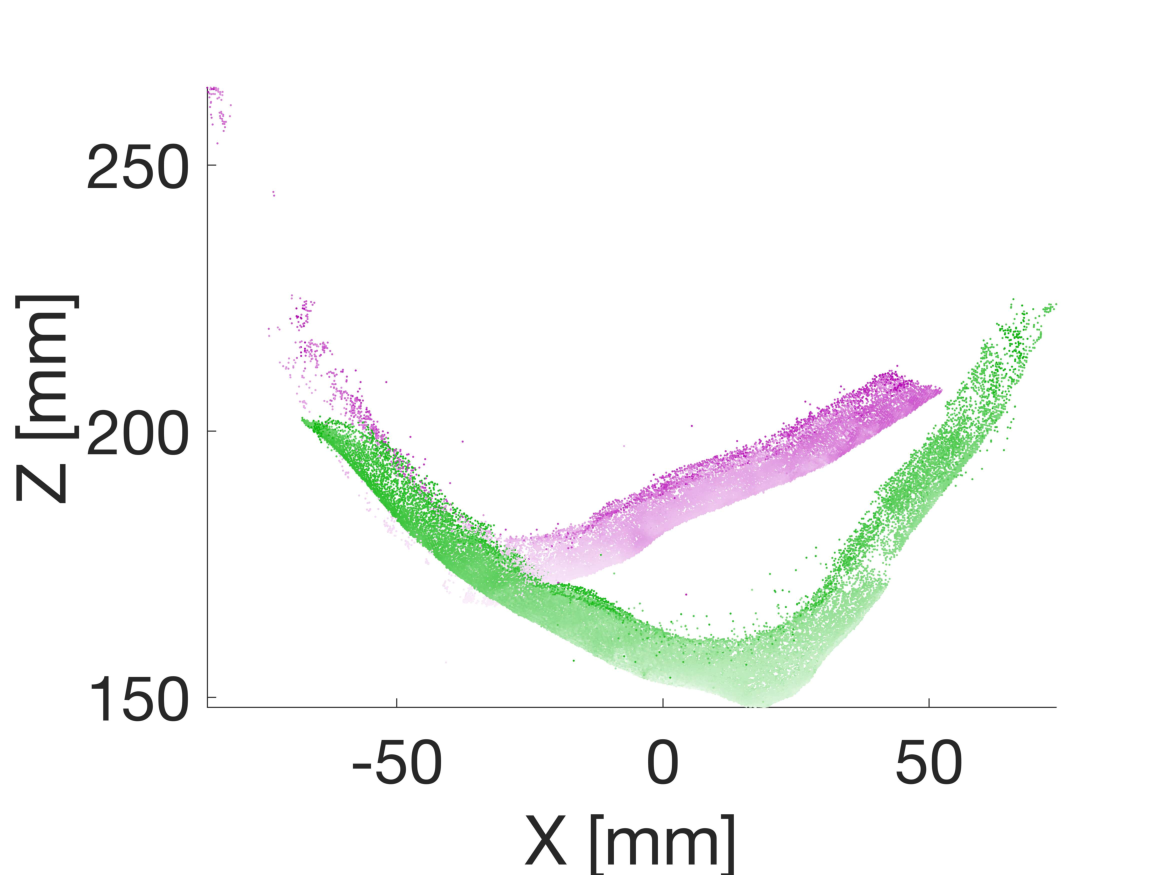
\includegraphics[width=0.32\textwidth]{PC_dual.pdf}}
	\subfigure[]{\label{fig:pcmergeb}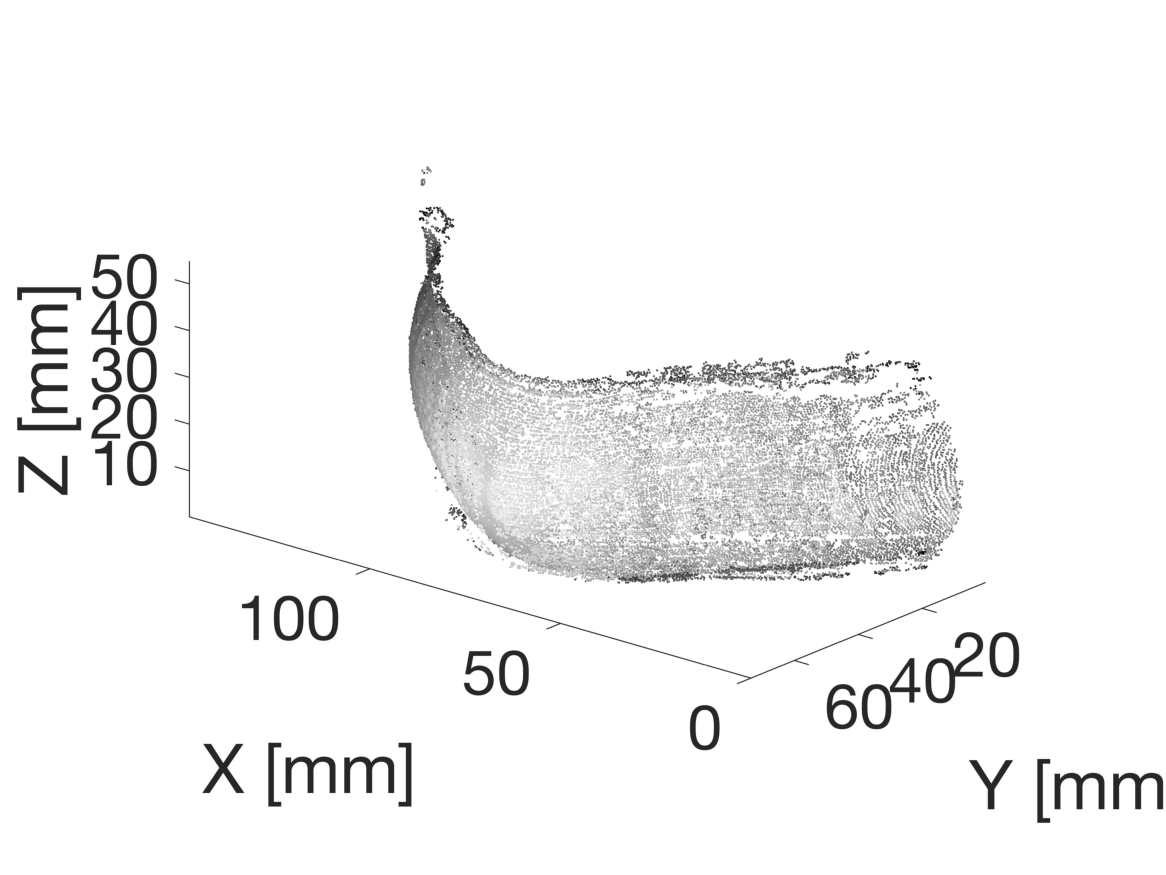
\includegraphics[width=0.32\textwidth]{PC_merged.pdf}}
	\end{center}
	\caption{(a) Surface mesh of a digital breast tomosynthesis model obtained from The Cancer Imaging Archive~\cite{Clark2013}. Blue cyan lines show the $x/y$ and $y/z$ breast contours from the top and side views. (b) Estimate of the DBT surface using the extrusion method in which the contour (cyan) is extruded to the thickness of the breast along the $z$ axis. (c) The top-sweep method uses the $x/y$ contour as the profile (cyan) and the $y/z$ contour as the path to sweep (red). (d) The side-sweep method uses the $y/z$ contour as the profile (cyan) and the $x/y$ contour as the path to sweep (red). (e) point-clouds from both camera-projector pairs were generated by scanning a 3-D printed model of the DBT breast using the SLI system. The green (Camera 1) and magenta (Camera 2) point-clouds are in the respective camera coordinates. (f) Merged and denoised point-cloud in the projector's coordinates.} 
	\label{fig:meshes}
\end{figure} 

\subsubsection{Structured light imaging surface mesh generation}
The SLI system estimates the surface of the compressed breast from the captured images while the breast is illuminated with Gray-code sequence patterns. Each camera-projector pair's extrinsic parameters are used to generate a point-cloud in each camera's reference frame using Scan3d-Capture~\cite{Moreno2012a} [Fig.~\ref{fig:pcmergea}]. The alignment of each camera-projector pair point-cloud is done by a rigid transformation of each point-cloud to the projector's coordinates. The point-clouds are then down-sampled using a box grid filter and merged to a single point with normal properties averaged~\cite{Pomerleau2013}. Denoising is then performed to remove outliers~\cite{Rusu2008}. The point-cloud is trimmed in the $z$ direction to the height of the DBT breast measured by the linear encoder [Fig.~\ref{fig:pcmergeb}]. The trimmed point-cloud is first converted to a mesh using a crust algorithm~\cite{Crust1999} prior to being cropped by a bounding-box mesh with height matching the breast thickness to form a closed surface mesh. 

\subsubsection{Surface estimation error}
The surface estimation error, $E_s$, of each surface estimation method is computed by comparing the nodes in each surface mesh to the nodes in the DBT mesh. The residual for each node in the surface mesh is the shortest distance from that node to the DBT mesh. The SLI output mesh is linearly translated (rotation and translation only) into the projector's frame using the projector's extrinsic parameters prior to determining residuals. $E_s$ is defined as the average residual of all nodes for a particular surface estimation method. 


%%% Subsection %%%
\subsection{Evaluation of the impact of surface errors on DOT image reconstructions}
Simulations were conducted to evaluate the impact of surface estimation accuracy on DOT reconstruction accuracy for inclusions of various depths. Breast surface meshes were converted to volumetric meshes with optical inclusions and the mean squared error of wide-field DOT reconstructions was calculated for each estimation method. 

\subsubsection{Assessment of reconstruction accuracy}
The effect of different surface estimations on lesion reconstruction was quantified using simulations of continuous wave (CW) pattern-illumination sources. A 5~mm radius spherical inclusion was added at the mid-plane of each volumetric mesh at distances of 5 to 45~mm away from the nipple. The $x$ and $z$ coordinates of the inclusion were fixed at 68 and 22~mm, respectively. The forward simulation was conducted on a ground truth volumetric mesh consisting of the DBT volumetric mesh and a spherical inclusion. The non-linear image reconstruction of tissue properties was calculated using an iterative Gauss-Newton method in which a series of corrective terms were added to an initial guess~\cite{Fang2009}. The reconstruction resulted in distributions, $\mathrm{\mu_{a}}_{i}$, representing the resulting 3-D absorption coefficient ($\mu_a$) maps at the $i^{th}$ node for each simulated tumor location and surface model.

\subsubsection{Reconstruction error assessment}
We use mean squared error, MSE, to determine the accuracy of the image reconstruction resulting from each breast mesh. To compute the MSE, we first interpolate the reconstructed absorption map, $\mu_a$, to the DBT mesh, and then subtract the interpolated $\mu_a$ at each node $i$, with the corresponding ground truth absorption value defined on the same node, expressed as
\begin{equation}
\label{eq:mse}
\mathrm{MSE} = \frac{1}{N}\sum_{i=1}^{N}(\mathrm{\mu_{a}}_{i} - \mathrm{\mu_{a0}}_i)^{2},
\end{equation}
where $N$ is the total node number; $\mathrm{\mu_{a}}_i$ and $\mathrm{\mu_{a0}}_i$ define the recovered and ground truth $\mu_{a}$ values, respectively, at the $i^{th}$ node in the DBT mesh.



\section{Results}
\label{chap:omci:results}



\section{Discussion}
\label{chap:omci:discussion}



% CONCLUSION GOES INTO THE CONLUSION OF THE ENTIRE THESIS

% --- EOF ---